\section{Simulación de la se\~nal}\label{sec:sig_samples}

\subsection{Generación de eventos}

La conexión entre la teoría/fenomenología de SUSY (o cualquier otra teoría de
nueva física), y los datos observados en el detector de un
colisionador se realiza por medio de un \hl{\emph{generador de eventos}}. Dada una
teoría de nueva física, que en general predice la existencia de nuevas
partículas y/o interacciones, el generador de eventos permite calcular cómo esa
teoría se manifiesta en el experimento\cite{Baer:2009tk}.

El procedimiento, una vez que se selecciona un modelo particular de SUSY,
requiere de varios pasos que se encuentran esquematizados en la
\cref{fig:mc_sketch}. En primer lugar es necesario calcular el espectro de masas
de las partículas supersimétricas, y sus acoplamientos. A partir de esto se
calculan los anchos y tazas de decaimiento de todas estas partículas. Y por
último se utiliza el generador, que toma como entrada las masas y decaimientos
calculados previamente, y genera los \hl{eventos de SUSY} a la energía de centro de
masa del colisionador. Para las distintas etapas suelen utilizarse herramientas
diferentes, por lo que es fundamental contar con un forma estandarizada de
intercambio de información entre ellas. Con este objetivo se creo un tipo de
archivo llamado SLHA (SUSY Les Houches Accord)\cite{SLHA} que permite organizar
toda la información de un cierto modelo de supersimetría (parámetros, masas,
decaimientos) en un unico formato y de modo que sea fácil de compartir entre los
físicos y también las distintas herramientas.

\begin{figure}[h]
  \centering
  \scalebox{0.8}{\begin{tikzpicture}[node distance=1.5cm, auto,]

    \node[rec] (susy) {\sc Modelo SUSY};
    \node[rec, right=of susy] (masses) {\sc Espectro de Masas};
    \node[rec, right=of masses] (decays) {\small \sc Decaimientos};
    \node[rec, right=of decays] (gen) {\sc Generador de Eventos};
    \node[rec, right=of gen] (atlas) {\sc Simulación Detector};

    \draw[arr] (1.7,0) -- (2.7,0);
    \draw[arr] (6.2,0) -- (7.2,0);
    \draw[arr] (10.8,0) -- (11.7,0);
    \draw[arr] (15.1,0) -- (16.1,0);

\end{tikzpicture}
}
  \caption{Etapas de la generación de eventos de un modelo de SUSY.}
  \label{fig:mc_sketch}
\end{figure}

%% Para interfacear dos o mas calculos, el procedimiento general requiere que
%% el usuario prepare los parametros del modelo ,
%% junto con un conjunto de parametros
%% del SM (que seran usados como las
%% condiciones de contorno a escala de baja energia para el calculo del espectro),
%% en un archivo de texto , siguiendo el acuerdo SLHA.

%% Luego se corre un generador de espectro con este archivo como entrada para obtener
%% las masas de las particulas SUSY y los acoplamientos a la escala electrodebil.
%% El espectro resultante es guardado, junto con una copia de los parametros de entrada)
%% en un nuevo archivo.

%% El siguiente paso es utilizar un programa que genere los modos de decaimiento y sus anchos
%% para las particulas seleccionadas, que se guarda en un tercer archivo, junto con la copia
%% de los parametros de entrada y el espectro de masas.

%% Y por ultimo, se utiliza un generador de eventos (completo o a nivel partonico) que
%% genera los eventos a partir de la informacion de este archivo.


\subsubsection{Espectro de masas y decaimientos}

Los modelos de SUSY que se estudian en el LHC suelen ser la teoría efectiva a
bajas energías que resultan de una teoría mas general, como teoría de
supercuerdas, o que involucre un mecanismo particular para el rompimiento de
SUSY. Para especificar una teoría efectiva es necesario definir: (1) la simetría
de gauge, (2) los campos que la componen y, (3) el Lagrangiano. Como se describio
en el \cref{cap:susy}, los efectos del
rompimiento de SUSY están codificados en los términos de rompimiento soft del
Lagrangiano.
También es necesario especificar la escala de energía a la cual la
teoría efectiva y el lagrangiano son válidos. Y como los experimentos prueban
física a la escala del {\tev}, mientras que los parámetros del
Lagrangiano son frecuentemente especificados a energías mucho mas altas
($M_\text{GUT}$ o $M_P$), debe usarse el grupo de ecuaciones de renormalización
(RGE) para conectar las dos escalas del modelo. Una vez que los parámetros del
Lagrangiano son conocidos a la escala electrodébil, pueden identificarse las
masas físicas de las partículas, diagonalizando las matrices de masa
correspondientes, y luego, para tener la precisión suficiente, aplicar las
correcciones a ordenes mayores (en general a 1 \hl{loop}). A partir del modelo
también es posible calcular los anchos y tazas de decaimiento de todas las
partículas supersimétricas.

Existe una gran variedad de programas que permiten realizar estos cálculos.
En este trabajo utilizamos el programa
{\susyhit}\cite{Djouadi:2006bz} que combina {\suspect}\cite{Djouadi2007426}
para calcular el espectro de masas, junto
con {\sdecay}\cite{Muhlleitner:2004mka} y {\hdecay}\cite{Djouadi:1997yw}
para calcular los BRs y anchos de decaimiento. Algunos de estos modos de
decaimientos son calculados a NLO en QCD.

%% {\suspect}\note{referencia} corre las RGE a dos loops en el MSSM para determinar
%% los parametros de SUSY a la escala electrodebil en modelos de mSUGRA, GMSB, AMSB
%% y pMSSM. Y aplica luego las correscciones a 1 loop, y algunas correcciones a 2 loops
%% para las masas de los Higgs.

Una vez que el espectro de masas y los decaimientos están calculados estos
pueden usarse como entrada en los generadores de eventos.

%% % SLHA
%% Para facilitar el intercambio de información entre distintos programas de SUSY
%% se propuso una seria de convenciones: SUSY Les Houches Accord (SLHA)\cite{SLHA}.
%% Este acuerdo permite usar la salida de los códigos que calculan el espectro de
%% masa y decaimientos como entrada en los generadores de eventos de una forma
%% consistente y sin ambigüedades.

%% %% En general estos modelos pueden
%% %% ser teorias efectivas
%% La teoria efectiva queda especificada adoptando la simetria de
%% gauge, the (super)field content y el Lagrangiano.
%% {\suspect} runs the 2-loop MSSM RGEs to determine weak scale
%% SUSY parameters in the mSUGRA, GMSB and AMSB models,
%% and in the pMSSM (a more general MSSM model). One-loop
%% sparticle mass corrections are included.
%% Some two loop corrections to Higgs masses are included.


\subsubsection{Generador de eventos}\note{Cambiar?}

Los programas descriptos anteriormente permiten pasar de un modelo de SUSY a las
predicciones en la producción de partículas y sus anchos de decaimientos en
estados finales de quarks, leptones, fotones y gluones (y LSP en modelos donde
se conserva paridad-R).
%% Sin embargo los quarks y gluones no pueden medirse
%% directamente en los detectores.
%% Los detectores pueden medir trazas de partículas
%% (cuasi)estables cargadas y su momento en campos magnéticos, como también los
%% depósitos de energía en los calorímetros.
Por lo tanto todavía falta un paso
entre estos modelos y las señales detectadas en los detectores, del cual se
encarga el generador de eventos. A partir de la colisión hadronica inicial,
estos programas modelan la producción de las partículas en el estado final a ser
medidas en el detector.

Para un dado tipo de colisionador y una dada energía de centro de masa, y un
modelo, el generador de eventos va a generar un conjunto eventos de pares de
spartículas de acuerdo a su sección eficaz. Estas partículas van a decaer
(posiblemente en en una cascada de varios pasos) en un estado final partónico,
de acuerdo a los BR fijados por el modelo. Este estado final partónico es
convertido en uno con partículas que puede ser detectadas en el detector.
Generando un gran número de eventos de SUSY, se pueden simular los posibles
estados finales que se espera a paritr de un un cierto modelo.

La simulación de las particulas producidas a partir de colisiones en
colisionadores hadrónicos puede descomponerse en varios pasos descriptos a
continuación (y esquematizados en la \cref{fig:mc_event_generator}):

\begin{itemize}

\item Interacción dura (HS):

  En este proceso, las partículas aceleradas (en este caso protones) interactúan
  para producir las partículas primarias salientes. La interacción dura
  involucra los partones de los hadrones intervinientes en el proceso. El
  cálculo se realiza, en general, a primer orden (LO) en teoría de
  perturbaciones, aunque algunos programas pueden incluir algunos procesos a
  NLO. Esta etapa también involucra la convolución con las funciones de
  distribución partónico (PDFs) para obtener las secciones eficaces de producción,

\item Cascadas partónicas:

  Implementación de las lluvias partónicas para las partículas producidas en la
  colisión (lluvia de estado final o FSR), para los partones iniciales
  involucrados en la colisión (lluvia de estado inicial o ISR), y también para
  otras partículas de color que puedan ser producidas como decaimiento de
  partículas mas pesadas.\note{Cambiar!}

  %% implementación de las lluvias de partones para los estados de partículas
  %% con color inicial y final, y para otras partículas con color que puedan ser
  %% producidas como decaimiento de otros objetos mas pesados,

\item Decaimientos:

  Las partículas supersimétricas producidas en la interacción dura decaen (en
  general en forma de cascada) a otras partículas.

  %% Las particulas fundamentales masivas, como el quark top,
  %%   los bosones de gauge electrodebiles, los bosones de Higgs y particulas de nueva fisica, decaen
  %%   en una escala de tiempo que es mas corta o comparable a las lluvias partinicas QCD.
  %%   Dependiendo de la naturaleza de las particulas y de si se producen particlas que interacctuen
  %%   fuertementen en el decaimiento, estas marticulas pueden tambien iniciar lluvias partonicas
  %%   antes y despues de su decaimiento.

\item Hadronización y produccion de particulas estables:

  En esta etapa se implementa el modelo de hadronización que describe la
  formación de mesones y bariones a partir de los quarks y gluones. También las
  partículas inestables deben decaer a partículas (cuasi) estables que son
  detectadas en el detector, con tasas y distribuciones que estén de acuerdo con
  los valores medidos o predichos.

\item Remanentes:

  Finalmente, los remanentes de los haces iniciales tienen que ser
  modelados para obtener una descripción válida de la física incluyendo
  no solo el HS sino los procesoso ``soft'', lo que suele llamarse evento subyacente (UE).

\end{itemize}

%% \begin{figure}[h]
%%   \centering
%%   \includegraphics[width=0.6\textwidth]{figures/mc_event_generator}
%%   \caption{Distintas etapas implementadas en los generadores de eventos Monte Carlo.
%%     (1) Interacción dura (HS), (2) Lluvias de estado inicial y final (ISR, FSR),
%%     (3) Decaimientos en cascada, (4) Hadronización, (5) Remanentes.}
%%   \label{fig:mc_event_generator}
%% \end{figure}

\begin{figure}[!htbp]
  \centering

  \scalebox{0.9}{%% \usetikzlibrary{positioning}
%% \usetikzlibrary{arrows}
%% \usetikzlibrary{patterns}
%% \usetikzlibrary{decorations.markings}
%% \usetikzlibrary{calc}
%% \usetikzlibrary{decorations}
%% \usetikzlibrary{decorations.pathmorphing}
%% \usetikzlibrary{decorations.pathreplacing}

\begin{tikzpicture}

  \tikzset{
    line/.style={line width=0.9},
    dline/.style={dashed,line width=0.9},
  }

  \definecolor{blue1}{HTML}{3F66BD}
  \definecolor{blue2}{HTML}{2C4784}

  %\draw[step=0.5,black!20,thin] (-5,-5) grid (5,5);
  %\draw[step=1,red!30,thin] (-5,-5) grid (5,5);

  \coordinate (p1) at (-2, 3);
  \coordinate (p2) at (-2,-3);
  \coordinate (O) at (2,0);

  \node at (-4, 3) {p};
  \node at (-4,-3) {p};

  \draw (-3.75, 3) -- (p1);
  \draw (-3.75,-3) -- (p2);

  \draw (0,-0.5) -- (0,0.5);
  \draw (p2) -- (0,-0.5);

  \draw[gluon] (p1) -- (-1.2, 2);
  \draw (-1.2,2) -- (-0.74,1.4);
  \draw[gluon] (-0.74,1.4) -- (-0.05, 0.55);
  \draw (-1.2,2) -- (-0.3, 2.5);
  \draw (-0.74,1.4) -- (0, 1.8);

  \draw[dashed] (0,-0.5) -- (2,-1);
  \draw         (0, 0.5) -- (2, 1);

  \draw (2,-1) -- (2.5,-1.5);
  \draw (2,-1) -- (4, 0);

  \draw[dashed] (3, -0.5) -- (3.5,-1);
  \draw (3.5, -1) -- (3.8, -1.50);
  \draw (3.5, -1) -- (4, -0.80);

  \draw[dashed] (2, 1) -- (3,2);
  \draw (2, 1) -- (2.5,0.5);

  \draw (-2,3) -- (-0.5,3.5);
  \draw (-2,3.1) -- (-0.5,3.7);

  \draw (-2,  -3) -- (-0.5,-3.5);
  \draw (-2,-3.1) -- (-0.5,-3.7);

  \draw[gluon] (-1.2,-2) -- (0,-2.5);
  \draw[gluon] (0,-2.5) -- (0.5,-2);
  \draw[gluon] (0,-2.5) -- (0.5,-3);
  \draw[gluon] (-0.55,-1.2) -- (0,-1.5);

  \draw (3,2) -- (3.5,2.5);
  \draw (3,2) -- (3.5,1.5);

  \draw[gluon] (3.5,-0.25) -- (4,-0.5);

  \node at (1,1.1) {$\tilde{g}$};
  \node at (1,-1.1) {$\tilde{q}$};
  \node at (4,-1.8) {$\tilde{\chi}^0_1$};
  \node at (3.9,1.5) {$\tilde{\chi}^0_1$};

  \draw[dashed,blue,line width=1] (0,0) circle(0.8);

  \node[blue] at (-1.75,0) {Interacción};
  \node[blue] at (-1.75,-0.5) {dura};

  \node[blue] at (0.1,2.0) {ISR, FSR};
  \node[blue,rotate=45] at (2.5,2) {Decaimientos};


  \draw[blue, decorate,decoration={brace,amplitude=4pt}] (4.2,0.23) -- (4.2,-0.55);
  \node[blue] at (5.6, -0.1) {Hadronización};

  \draw[blue, decorate,decoration={brace,amplitude=4pt}] (-0.2,-3.2) -- (-0.2,-4);
  \node[blue] at (1,-3.6) {Remanentes};

  \draw[fill=white] (p1) circle(0.25);
  \draw[fill=white] (p2) circle(0.25);

\end{tikzpicture}
}

  \caption{Distintas etapas implementadas en los generadores de eventos.}
  \label{fig:mc_event_generator}

\end{figure}

%% \note{del manual de Herwig}
%% Los procesos involucrados pueden dividirse en un número de etapas
%% correspondientes al aumento de las escalas de  tiempo y distancia
%% involucradas:

%% \item Lluvias de partones de estado inicial y final:
%%     Las particulas de color en el evento son perturvativamente evolucionadas desde
%%     la escala dura de la colision hasta el corte infrarojo.
%%     Esto ocurre para las particulas producidas en la colision, la \emph{lluvia de estado final},
%%     y los partones iniciales involucrados en la colision, la \emph{lluvia de estado inicial}.
%%     La coherencia de la emision de gluones soft en las lluvias de partones de las particulas en
%%     la colision dura es controlada por el flujo de color de la colision dura.

%%     %% 3. Decay of heavy objects. Massive fundamental particles such as the top quark, electroweak
%%     %% gauge bosons, Higgs bosons, and particles in many models of physics beyond the Standard
%%     %% Model, decay on time-scales that are either shorter than, or comparable to that of the QCD
%%     %% parton shower. Depending on the nature of the particles and whether or not strongly interacting
%%     %% particles are produced in the decay, these particles may also initiate parton showers
%%     %% both before and after their decay. One of the major features of the Herwig++ shower
%%     %% algorithm is the treatment of radiation from such heavy objects in both their production
%%     %% and decay. Spin correlations between the production and decay of such particles are also
%%     %% correctly treated.
%%   \item Decaimiento de objetos pesados: Las particulas fundamentales masivas, como el quark top,
%%     los bosones de gauge electrodebiles, los bosones de Higgs y particulas de nueva fisica, decaen
%%     en una escala de tiempo que es mas corta o comparable a las lluvias partinicas QCD.
%%     Dependiendo de la naturaleza de las particulas y de si se producen particlas que interacctuen
%%     fuertementen en el decaimiento, estas marticulas pueden tambien iniciar lluvias partonicas
%%     antes y despues de su decaimiento.

%%   \item

%%     4. Multiple scattering. For large centre-of-mass energies the parton densities are probed in a
%%     kinematic regime where the probability of having multiple partonic scatterings in the same
%%     hadronic collision becomes significant. For these energies, multiple scattering is the dominant
%%     component of the underlying event that accompanies the main hard scattering. These
%%     additional scatterings take place in the perturbative regime, above the infrared cut-off, and
%%     therefore give rise to additional parton showers. We use an eikonal multiple scattering
%%     model [8], which is based on the same physics as the FORTRAN JIMMY package [18], together
%%     with some minor improvements. In addition to that we included non-perturbative
%%     partonic scatters below the infrared cut-off [19], which enables us to simulate minimum
%%     bias events as well as the underlying event in hard scattering processes.

%%     5. Hadronization.
%%     After the parton showers have evolved all partons involved in hard scatterings,
%%     additional scatters and partonic decays down to low scales, the final state typically
%%     consists of coloured partons that are close in momentum space to partons with which they
%%     share a colour index, their colour ‘partner’ (in the large Nc limit this assignment is unique).
%%     Herwig++ uses the cluster hadronization model [2] to project these colour–anticolour pairs
%%     onto singlet states called clusters, which decay to hadrons and hadron resonances. The
%%     original model of Ref. [2], which described this decay as pure phase space has been progressively
%%     refined as described in Sect. 7. Clusters that are too massive or too light for decay
%%     directly to hadrons to provide a good description are treated differently, again described in
%%     Sect. 7.

%%     6. Hadron decays. The hadron decays in Herwig++ are simulated using a matrix element
%%     description of the distributions of the decay products, together with spin correlations between
%%     the different decays, wherever possible. The treatment of spin correlations is fully
%%     integrated with that used in perturbative production and decay processes so that correlations
%%     between the production and decay of particles like the tau lepton, which can be
%%     produced perturbatively but decays hadronically, can be treated consistently.


\subsubsection{Funciones de distribución partónica}

Las funciones de distribución partónica (PDFs) se utilizan para describir la
subestructura del protón y son usadas por todos los generadores de eventos.
ATLAS utiliza la librería LHAPDF\cite{Bourilkov:2006cj} que contiene un
repositorio con una gran
cantidad de PDFs. Por defecto, y a menos que se indique lo contrario las PDFs
CTEQ son las utilizadas en ATLAS.


\subsubsection{Simulación del detector ATLAS}

Para poder estudiar la respuesta del detector para un gran número de procesos
físicos y escenarios, se ha implementado una simulación detallada que lleva los
eventos de la generación a un formato que es idéntico a las señales en el
detector verdadero\cite{AtlasSim}. La simulación esta integrada al software de
ATLAS (\textsc{Athena}), y utiliza el paquete de simulación
{\geant}4\cite{Geant4}.

La simulación esta dividida en tres etapas: (1) generación del evento y los
decaimientos inmediatos, (2) simulación del detector, y (3) digitalización de
los depósitos de energía en las regiones sensibles del detector en los voltajes
y corrientes que se encuentran a la salida del detector. Luego, la salida de
estos procesos de simulación sirve como entrada a los algoritmos de
trigger y reconstrucción de ATLAS, que son idénticos a los que se utilizan en
los datos reales.

Existe también una simulación rápida del detector que es utilizada en los casos
donde no es necesaria un simulación tan minuciosa de las lluvias
electromagnéticas en los calorímetros. Casi 80\% del tiempo de simulación se
debe a la simulación de partículas atravesando el calorímetro, y cerca del 75\%
se emplea en la simulación de las partículas electromagnéticas. En la simulación
rápida \textsc{Atlfast}\cite{Richter-Was:683751}, se remueven estas partículas
electromagnéticas de baja energía y se las reemplaza con lluvias
electromagnéticas pre-simuladas. De esta forma se reduce el consumo de CPU
notablemente considerando las características de la física en cuestión.


\subsubsection{Pile-up}
\label{sec:prw}

Las muestras MC son generadas utilizando las condiciones esperadas del LHC y
ATLAS para la toma de datos, ya que se suelen generar previo a la toma de datos.

Por lo tanto, existen algunas diferencias entre datos y las muestras MC. Para
solucionar esto a las muestras MC se les aplica un repesado evento a evento
para modelar las condiciones reales de los muestras de datos. Los pesos
utilizados se calculan de modo de

%% Como las muestras MC son por lo general generadas antes de la toma de datos,
%% se utilizan las condiciones esperadas del acelerador y el detector.
%% Por lo tanto, despues de la toma de datos se encuentran diferencias

Un repesado evento a eventos es aplicado a todas las muestras MC para modelar las condiciones
realistas de las muestra de datos bajo estudio, matcheando la distribución del número de interaccionas
por cruze de bunchs (pile-up) de las muestras simuladas a la observada en datos\note{fix}.

%% ---
%% Cada evento en una muestra Monte Carlo es producido bajo ciertas condiciones particulares del detector, y bajo un valor particular de pile-up.
%% Cada condicion del detector le corresponde una distribucion  de pile-up distinta, que es utilizada para determinar el valor de pile-up que
%% tiene que ser usado para simular cada evento de la muestra. Los valores simulados de pile-up forman entonces un conjunto discreta, a
%% diferencia de los datos en los que el valor de pile-up es una variable continua.
%% --


%% Monte Carlo (MC) event samples, including a full simulation
%% [10] of the ATLAS detector within geant4 [11],
%% are used to compare the data to the SM signal and background
%% expectations. All MC samples are simulated with
%% in-time pile-up (an average of four pp interactions within
%% a single bunch crossing) and out-of-time pile-up (signals
%% from neighbouring bunch crossings). The simulated
%% events are weighted such that the distribution of multiple
%% collisions per bunch crossing matches what is observed in
%% the data for the period used in this analysis.



%-------
% Senal
%-------
\subsection{Se\~nal}

Como se ha mencionado en el \cref{cap:susy}, debido al gran número de parámetros
libres en los modelos de SUSY, las búsquedas de supersimetría en ATLAS están
impulsadas por la fenomenología de los estados finales. El análisis realizado
para esta Tesis esta motivado por los estados finales con fotones
energéticos, provenientes del decaimiento de un neutralino NLSP en el contexto
de modelos GGM.

En los modelos GGM el decaimiento de los estados supersimétricos producidos
durante las colisiones van a proceder por medio de decaimientos en cascada hasta
el neutralino NLSP que decaerá a un gravitino y una partícula del SM,
que dependerá de la naturaleza de la NSLP. Distintas posibilidades para la
naturaleza de la NLSP fueron consideradas, las cuales dan lugar y motivan
estados finales distintos y complementarios entre si, para cubrir las distintas
regiones del espacio de fase de los modelos GGM. Dentro de ATLAS, distintos
analisis exploraron cuatro estados finales diferentes: dos fotones, un fotón y
un leptón, un fotón y {\bjets}, y un fotón y jets, todos con energía faltante,
correspondiente a los gravitinos LSP.

En particular en esta Tesis se describe el análisis de un estado final que
consiste en un único fotón, jets y energía faltante.
La selección de eventos descripta en el \cref{cap:seleccion} fue diseñada para
maximizar la sensibilidad a pequeñas señales con esta topología general.
Cualquier imposición de cortes muy dependientes del modelo fueron evitadas,
tratando de mantener el análisis lo mas independiente del modelo como fuera
posible. Sin embargo, una interpretación en el marco de un modelo especifico es
inevitable. Con tal motivo se simuló un conjunto de puntos de señal con
distintos valores de los parámetros para cubrir la región del espacio de
parámetros donde pueda manifestarse dicha señal.

%% Se simularon puntos de senal para la produccion de gluinosLos resultados se interpretaron
%% son interpretados en el contexto de GGM que
%% incluyen la produccion de supercompaneras de particulas del SM que se acoplan
%% fuertemente comot ambien de que poseen solo carga electrodebil.

Se utilizó un espectro simplificado, en el cual, básicamente, el espacio de
parámetros consiste en la escala de producción (por simplicidad, la masa del
gluino) y la masa de la NLSP. Todos los demás estados fueron desacoplados ya que
no juegan un rol importante en la producción o en el estado final de interés.
Esta aproximación es similar a los denominados \emph{modelos simplificados}
utilizados en otras búsquedas.
La masa del gluino es el único parametro libre de las partículas de color, para
poder determinar un límite conservativo en la masa del mismo. Todos los
parámetros de masa soft de los squarks se fijan en 2.5 \tev.

Para maximizar la probabilidad de tener un único fotón en el estado final, es
necesario que $\mathrm{BR}(\ninoone \to \gam\,\gravino) \sim 50\%$. Esto resulta
cuando el neutralino mas liviano es una mezcla bino-higgsino.
Además, el valor de $\mu$ debe ser positivo para
suprimir el decaimiento a Higgs, que llevara a un estado final ya cubierto por
otro análisis de ATLAS.
Para lograr la BR
deseada, para las diferentes masas del {\ninoone}, se variaron los parámetros de
masa de bino ($M_1$) y higgsinos ($\mu$), de tal forma que los BR del {\ninoone}
sean aproximadamente constantes:

\begin{align}
  &\mathrm{BR}(\ninoone \to \gam\, \gravino) \approx 50\% \label{eq:n1_gam}\\
  &\mathrm{BR}(\ninoone \to Z\, \gravino) \approx 49\%    \label{eq:n1_z} \\
  &\mathrm{BR}(\ninoone \to h\, \gravino) \approx 1\%     \label{eq:n1_h}
\end{align}


Los demás parámetros del modelo se fijan en $M_2=2.5\tev$, $\tan\beta=1.5$ y
$c\tau_{\mathrm{NLSP}} < 0.1$ mm. Este último asegura que el neutralino decaiga
rápidamente dentro del detector y se logra haciendo al gravitino lo
suficientemente liviano ($m_{\tilde{G}}=10^{-9} \gev$). Todos los términos
tri-lineares son fijados a cero y las masas de los sleptones a $2.5 \tev$.
Las masas del higgs liviano ($h$) y el pseudoescalar ($A$) se fijan a
$m_{A} = 2 \tev$ y $m_{h} = 126 \gev$.
La masa del $h$ se considera a partir del valor
medido de la masa del Higgs observado en el ano 2012.
En modelos GGM de SUSY existen distintos
mecanismos\cite{Craig:2011yk,Auzzi:2011eu,Csaki:2012fh,Larsen:2012rq,Craig:2012hc}
para generar una masa del bosón de Higgs tan alta como este valor observado, sin
cambiar la fenomenología de los modelos considerados. No se vio un efecto
significativo en el espectro de masa variando el valor de la masa de Higgs en un
rango de $\pm 10 \gev$.\note{Hacer comentario de $\tan\beta$}

A partir de estos estudios se simuló un conjunto de puntos de señal (grid) en el plano
($m_{\gluino}$, $m_{\ninoone}$), variando los parámetros $M_3$ y $\mu$. Y $M_1$
se ajusto, dependiendo del $\mu$ de forma de obtener las BR descriptas
anteriormente. La grid cubre el espacio $150\gev < m_{\ninoone} < 1250 \gev$ y
$800\gev < m_{\gluino} < 1300 \gev$, con $m_{\ninoone} < m_{\gluino}$ (ver
\cref{fig:gridpoints}).


\begin{figure}[!htbp]
  \centering
  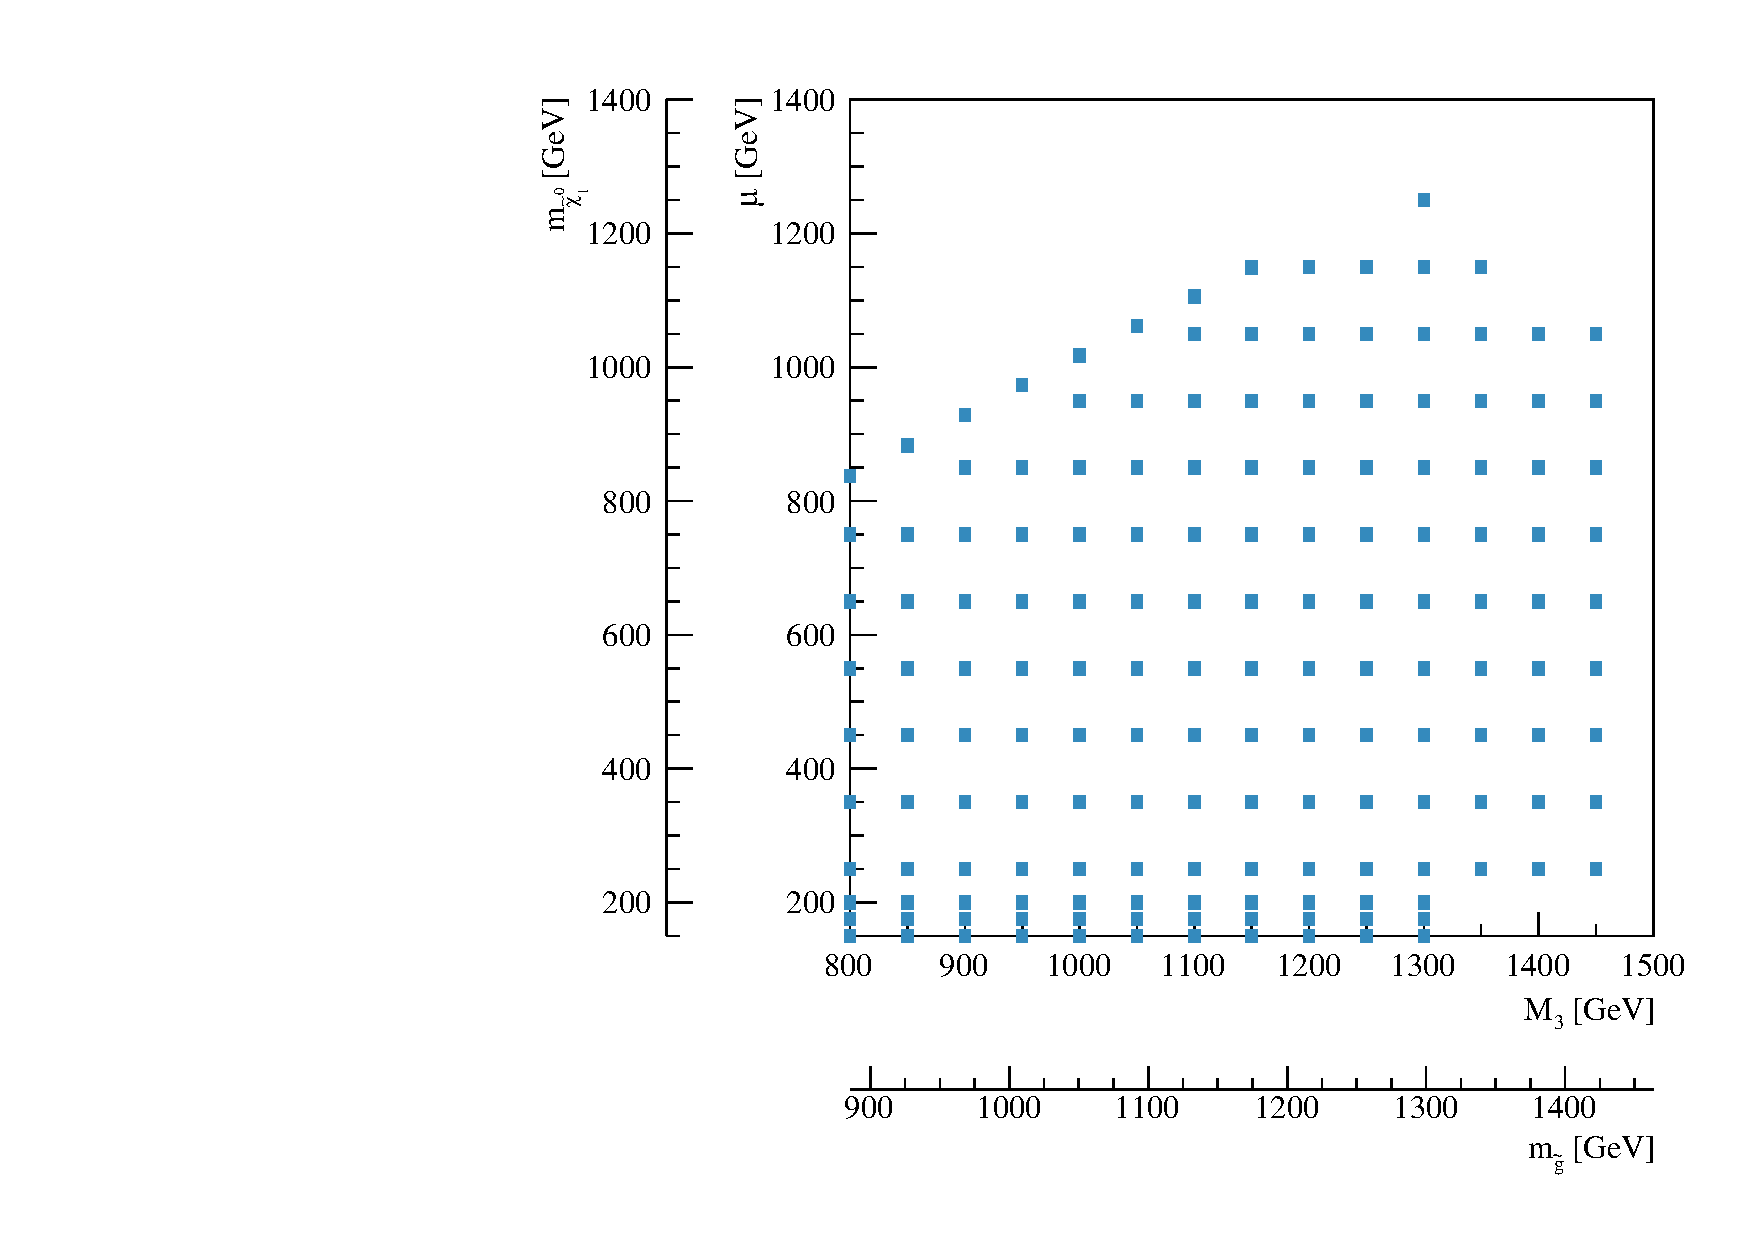
\includegraphics[width=0.5\textwidth]{figures/run1_grid}
  \caption{Update plot!}
  \label{fig:gridpoints}
\end{figure}


El espectro completo de masas y los correspondientes decaimientos fueron
calculados a partir de estos parámetros utilizando {\suspect}
(v2.41)\cite{Djouadi2007426}, {\sdecay} (v1.3b)\cite{Muhlleitner:2004mka} y
{\hdecay} (v3.4)\cite{Djouadi:1997yw}, que forman parte del paquete {\susyhit}
(v1.3)\cite{Djouadi:2006bz}. Algunos ejemplos del espectro de masas puede verse
en la \cref{fig:mass_spectra}, para algunos puntos de la grid.

\begin{figure}[!htbp]
   \centering
   \includegraphics[width=0.45\textwidth]{figures/masses_GGM_M3_mu_800_150}
   %%\includegraphics[width=0.45\textwidth]{figures/masses_GGM_M3_mu_1000_750}
   \includegraphics[width=0.45\textwidth]{figures/masses_GGM_M3_mu_1450_1050}

   \caption{Espectro de masas de las particulas supersimetricas para dos puntos de la grid de senal.
     En la izquierda para XXX y en la derecha XXX.}
     %% Solo $M_3$ y $\mu$ son los parámetros libres, en este caso
     %% $(M_3, \mu) = (800~\gev, 250~\gev)$. }
   \label{fig:mass_spectra}
\end{figure}

Para cada uno de los 124 puntos de señal que constituyen la grid se generaron
5000 eventos, utilizando {\herwigpp} v2.5.2\cite{Bahr:2008pv} y el conjunto de
PDFs CTEQ6L1\cite{Nadolsky:2008zw}. Se aplicó un filtro a nivel generador, que
requería la presencia de un fotón con un {\pt} de al menos 100 \gev, para
obtener mas estadística\note{Aclarar}, especialmente en los puntos donde el
neutralino tiene menor masa. La eficiencia del filtro para todas las muestras
simuladas puede verse en la \cref{tab:signal_filter_eff}. La simulacion del
detector ATLAS se realizo con la simulación rápida
\textsc{ATLFAST-II}\cite{Richter-Was:683751}.



\begin{table}[!htbp]
  \centering
  \caption{Relación entre los parámetros libres del modelo $M_3$ y $\mu$ con las
    masas $m_{\gluino}$ (izquierda) y $m_{\ninoone}$ (derecha), respectivamente.
    En la tabla de la derecha, para cada valor de $\mu$ también se puede
    observar el valor de $M_1$ utilizado para obtener los BR de decaimiento del
    {\ninoone} deseados.}
  \label{tab:signal_pars}

  \begin{minipage}[!t]{0.5\textwidth}
    \centering
    \begin{tabular}{cc}
      \hline
      $M_3$ [\gev]& $m_{\gluino}$ [\gev] \\
      \hline
      800  & 885.5 \\
      850  & 931.7 \\
      900  & 977.6 \\
      950  & 1023.1 \\
      1000 & 1068.3 4  \\
      1050 & 1113.3 2  \\
      1100 & 1157.9 6  \\
      1150 & 1202.3 3  \\
      1200 & 1246.4 0  \\
      1250 & 1290.3 4  \\
      1300 & 1333.9 7  \\
      1350 & 1377.3 7  \\
      1400 & 1420.5 2  \\
      1450 & 1463.4 6  \\
      \hline
    \end{tabular}
    \vspace{5cm}
  \end{minipage}%
  \begin{minipage}[t]{0.5\textwidth}
    \begin{tabular}{ccc}
      \hline
      $\mu$ [\gev]& $M_1$ [\gev]& $m_{\ninoone}$ [\gev] \\
      \hline
      150  &  300  & 147.0  \\
      175  &  270  & 168.3  \\
      200  &  267  & 190.3  \\
      250  &  288  & 235.8  \\
      350  &  365  & 332. \\
      450  &  456  & 433. \\
      550  &  551  & 535. \\
      650  &  647  & 638. \\
      750  &  745  & 742. \\
      838  &  837  & 836. \\
      850  &  845  & 846. \\
      883  &  882  & 883. \\
      928  &  926  & 930. \\
      950  &  942  & 949. \\
      973  &  970  & 976.6  \\
      1017 &  1015 & 1023.4 \\
      1050 &  1040 & 1053.0 \\
      1062 &  1058 & 1068.9 \\
      1106 &  1102 & 1114.8 \\
      1149 &  1145 & 1160.0 \\
      1150 &  1140 & 1157.5 \\
      1250 &  1238 & 1260.6 \\
      \hline
    \end{tabular}

  \end{minipage}

\end{table}



%% \M{1} and $\mu$ determine the lightest neutralino mass, and are related in such a way that the branching ratios of the \ninoone\ are approximately constant,
%% resulting in ${\rm BR}(\ninoone \to \gam + \gravino) \approx 50\%$, ${\rm BR}(\ninoone \to Z + \gravino) \approx 49\%$ and ${\rm BR}(\ninoone \to h + \gravino) \approx 1\%$,
%% numbers which vary by $\pm 1\%$ throughout most of the grid ({\fig} \ref{fig:br_n1_x_grav}). For light neutralinos ($<200\gev$) the Higgs production is highly
%% suppressed and ${\rm BR}(\ninoone \to \gam + \gravino)$ starts falling up to 40\%. The value of $\mu$ must also be positive in order to disfavor the branching ratio
%% to the Higgs boson, which would lead to a signature already covered by a dedicated analysis in ATLAS \cite{Aad:2012jva}. Similarly, the branching ratio for
%% ($\ninoone \to \gam + \gravino$) is such that maximizes the single photon final state. At larger values the diphoton topology starts to be favoured, which has been
%% extensively searched for in the past \cite{Aad2012519,Aad:2011kz}. This leaves $M_3$ and $\mu$ as the only two free parameters of the model, spanning the space
%% within $150\gev < m_{\ninoone} < 1250 \gev$ and $800\gev < m_{\gluino} < 1300 \gev$, with $m_{\ninoone} < m_{\gluino}$. The granularity of the simulation in each
%% dimension is shown in {\tab}\ \ref{tab:signal_pars}, with the resulting value for the gluino and neutralino masses.




%%The total decay branching ratios for \gluino-initiated \ninoone\ production are
%% shown in {\fig} \ref{fig:br_gl_n1}, for 2-body\footnote{only effectively, the gluino decays through a virtual
%% quark-squark loop in this case.} and 3-body gluino decays.


\begin{table}[ht]
  \centering
  %\small
  \footnotesize
  \caption{Eficiencia del filtro a nivel generador [\%]
    para los puntos de señal simulados.}
  \begin{tabular}{c|ccccccccccccccccc}
    \hline
%       &    \multicolumn{11}{c}{Filter efficiency [\%]} \\
%	\hline
     &   \multicolumn{14}{c}{ $M_3$ [\gev] } \\
    $\mu$ [\gev] &  800 & 850 & 900 & 950 & 1000 & 1050 & 1100 &1150 & 1200  & 1250 & 1300 & 1350 & 1400 & 1450 \\
    \hline
    150  &   39.54 &   39.8 &  41.9    &   42.6   &   43.0   &   44.2   &   45.5    &   46.3    &    47.1  &   48.3  &   49.1 &      &      &       \\
    175  &   44.55 &   44.6 &  46.5    &   47.5   &   47.8   &   48.9   &   50.3    &   51.4    &    51.5  &   52.4  &   53.3 &      &      &       \\
    200  &   47.66 &   48.4 &  50.1    &   50.6   &   52.0   &   52.8   &   53.8    &   55.0    &    55.0  &   56.2  &   56.0 &      &      &       \\
    250  &   55.09 &   56.0 &  56.1    &   57.1   &   56.7   &   58.0   &   58.9    &   59.5    &    60.5  &   60.7  &   61.2 & 62.1 & 62.2 &  63.9 \\
    350  &   65.82 &   66.1 &  64.6    &   65.8   &   66.4   &   66.7   &   66.5    &   67.7    &    67.4  &   67.6  &   67.8 & 68.0 & 69.2 &  68.4 \\
    450  &   71.29 &   71.4 &  71.4    &   71.8   &   72.1   &   72.5   &   72.0    &   72.6    &    72.1  &   72.5  &   73.4 & 72.9 & 72.2 &  73.4 \\
    550  &   73.08 &   72.5 &  73.3    &   73.7   &   74.6   &   74.3   &   75.0    &   74.8    &    74.2  &   74.7  &   75.6 & 75.7 & 74.9 &  75.3 \\
    650  &   69.78 &   72.0 &  73.2    &   74.1   &   75.6   &   76.2   &   75.9    &   75.8    &    77.0  &   77.0  &   76.2 & 76.7 & 77.1 &  76.6 \\
    750  &   47.69 &   60.2 &  66.9    &   70.4   &   73.4   &   74.0   &   75.9    &   76.5    &    77.1  &   77.3  &   76.3 & 77.9 & 77.2 &  77.0 \\
    838  &    9.0  &        &          &          &          &          &           &           &          &         &        &      &      &       \\
    883  &         &   9.1  &          &          &          &          &           &           &          &         &        &      &      &       \\
    850  &         &        &  34.2    &   50.7   &   60.1   &   66.4   &   70.4    &   73.5    &    73.6  &   75.4  &   76.6 & 77.1 & 78.2 &  76.8 \\
    928  &         &        &   9.4    &          &          &          &           &           &          &         &        &      &      &       \\
    950  &         &        &          &          &   25.4   &   41.4   &   54.0    &   62.2    &    66.8  &   70.9  &   75.2 & 75.9 & 78.1 &  77.2 \\
    973  &         &        &          &   10.0   &          &          &           &           &          &         &        &      &      &       \\
    1017 &         &        &          &          &   10.3   &          &           &           &          &         &        &      &      &       \\
    1050 &         &        &          &          &          &          &   19.2    &   31.6    &    45.2  &   56.8  &   62.7 & 68.9 & 73.1 &  75.6 \\
    1062 &         &        &          &          &          &   11.1   &           &           &          &         &        &      &      &       \\
    1106 &         &        &          &          &          &          &   11.7    &           &          &         &        &      &      &       \\
    1149 &         &        &          &          &          &          &           &   12.6    &          &         &        &      &      &       \\
    1150 &         &        &          &          &          &          &           &           &    16.1  &   24.9  &   36.9 & 49.0 &      &       \\
    1250 &         &        &          &          &          &          &           &           &          &         &   16.1 &      &      &       \\
    \hline
  \end{tabular}
  \label{tab:signal_filter_eff}
\end{table}




\subsection{Sección eficaz de producción}
\label{sec:xs_calc}
%% La seccion eficaz de produccion y sus incertezas fue calculada usando el paquete SUSYSignalUncertainties \cite{SUSYsigunc}.
%% La seccione eficaz para los procesos que in volucran la produccion de pares de gluinos fueron calculadas a NLO
%% en la constante de acoplamiento fuerte, agregando la \hl{resummation of soft gluon emission at NLO+NLL}\cite{Beenakker:1996ch,Kulesza:2008jb,Kulesza:2009kq,Beenakker:2009ha,Beenakker:2011fu}.
%% La seccion eficas de produccion electrodebil de $\tilde{\chi}\tilde{\chi}$ fue calculada
%% a NLO en la constante de acoplamiento fuerte utilizando {\prospino} \cite{Beenakker:1999xh}.
%% Las secciones eficacez y sus incertezas estan detalladas en la \cref{tab:signal_xs_strong,tab:signal_xs_ewk}
%% y se muestran en las figuras...

En el caso de procesos de producción de pares de gluinos o squarks, de los cuales
existe el cálculo a NLL, la sección eficaz se toma a NLO en la constante de acoplamiento
fuerte, y se incluye la suma de la emisión de gluones soft con precisión NLL,
realizada utilizando {\nllfast}\cite{Kramer:2012bx,Beenakker:1996ch,Kulesza:2008jb,Kulesza:2009kq,Beenakker:2009ha,Beenakker:2011fu}
.

En el caso de la producción de otro tipo de procesos, como la producción electrodébil, se utiliza
las secciones eficaces calculadas a NLO usando {\prospino}.


\newcommand{\pdfcteqpm}{\ensuremath{\Delta\mathrm{PDF}^{\pm}(\mathrm{CTEQ})}}
\newcommand{\scacteqpm}{\ensuremath{\Delta\mathrm{SCA}^{\pm}(\mathrm{CTEQ})}}

\newcommand{\pdfmstwpm}{\ensuremath{\Delta\mathrm{PDF}^{\pm}(\mathrm{MSTW})}}
\newcommand{\scamstwpm}{\ensuremath{\Delta\mathrm{SCA}^{\pm}(\mathrm{MSTW})}}

\newcommand{\alphap}{\ensuremath{\alpha_s_+}}
\newcommand{\alpham}{\ensuremath{\alpha_s^-}}
\newcommand{\alphapm}{\ensuremath{\alpha_s^{\pm}}}

Las incertezas debidas a la elección de la escala de renormalizacion y
factorizacion como también de la PDF, son obtenidas utilizando {\nllfast} o
calculadas con {\prospino}. A fin de combinar todas estas predicciones y obtener
una incerteza total, se sigue las recomendaciones PDF4LHC\cite{Botje:2011sn}.
Para esto se define la envolvente de las predicciones a la sección eficaz usando
el intervalo a 68\% CL del conjunto de PDFs CTEQ (incluyendo la incerteza en
$\alpha_s$) y MSTW, junto con las variaciones de las escalas. La sección eficaz
nominal se obtiene usando el punto medio de la envolvente y la incerteza como la
mitad del ancho de la misma. Matemáticamente si {\pdfcteqpm} y {\scacteqpm} son
las variaciones en $\pm 1\sigma$ de las PDF CTEQ,  {\pdfmstwpm} y {\scamstwpm}
son las variaciones en $\pm 1\sigma$ en la PDF MSTW. Y {\alphapm} son las
correspondientes incertezas de la constante de acoplamiento fuerte. Entonces,

\begin{align}
  \Delta\mathrm{CTEQ}^{\pm} &= \sqrt{(\pdfcteqpm)^2 + (\scacteqpm)^2 + (\alphapm)^2} \\
  \Delta\mathrm{MSTW}^{\pm} &= \sqrt{(\pdfmstwpm)^2 + (\scamstwpm)^2}
\end{align}

Los correspondientes extremos por arriba y abajo de la envolvente pueden calcularse a partir de estos:

\begin{align}
  U &= \max(\Delta\mathrm{CTEQ}^\mathrm{nom} + \Delta\mathrm{CTEQ}^{+},\quad \Delta\mathrm{MSTW}^\mathrm{nom} + \Delta\mathrm{MSTW}^{+}) \\
  L &= \min(\Delta\mathrm{CTEQ}^\mathrm{nom} - \Delta\mathrm{CTEQ}^{-},\quad \Delta\mathrm{MSTW}^\mathrm{nom} - \Delta\mathrm{MSTW}^{-})
\end{align}
%
y la sección eficaz final ($\sigma$) y su incerteza simétrica ($\Delta\sigma$) se obtiene como:

\begin{equation}
  \sigma = (U+L)/2,\quad \Delta\sigma = (U-L)/2
\end{equation}


En la \cref{tab:signal_xs_strong} puede verse la sección eficaz de producción de
pares de gluinos para los distintos puntos de la grid de señal generada. La
sección eficaz de producción de neutralinos/charginos se encuentra en la
\cref{tab:signal_xs_ewk}. En la \cref{fig:signal_xs} también se encuentra
graficada la sección eficaz como función de la masa de las partículas
producidas, mientras que en la \cref{fig:signal_xs_total} se puede apreciar la
fracción en la producción electrodébil en comparación con la producción total.

\begin{table}[!htbp]
  \centering
  \caption{Sección eficaz a NLO+NLL para la producción de gluinos para los distintos
    puntos de la grid de señal. La ultima columna es la incerteza teórica.}
  \begin{tabular}{cccc}
    \hline
    $M_3$ [\gev] & $m_{\gluino}$ [\gev] & $\sigma$(NLO+NLL) [fb] & Incerteza Total [$\%$]\tabularnewline
    \hline
    800  &  885.5  & 69.05 & 22.5  \\
    850  &  931.7  & 44.92 & 23.8  \\
    900  &  977.6  & 29.73 & 25.2  \\
    950  &  1023.1 & 19.83 & 26.5  \\
    1000 &  1068.3 & 13.41 & 27.7  \\
    1050 &  1113.3 & 9.10 & 29.0  \\
    1100 &  1157.9 & 6.28 & 30.4  \\
    1150 &  1202.3 & 4.32 & 32.0  \\
    1200 &  1246.4 & 3.01 & 33.7  \\
    1250 &  1290.3 & 2.10 & 35.2  \\
    1300 &  1333.9 & 1.48 & 36.7  \\
    1350 &  1377.3 & 1.05 & 38.2  \\
    1400 &  1420.5 & 0.74 & 39.8  \\
    1450 &  1463.4 & 0.53 & 41.5  \\
    \hline
  \end{tabular}
  \label{tab:signal_xs_strong}
\end{table}

\begin{table}[!htbp]
  \centering
  \caption{Sección eficaz total a NLO para la producción electrodébil de neutralinos y charginos
    para los distintos puntos de la grid de señal. La última columna  es la incerteza
    teórica. Mas detalles se encuentran en la \cref{sec:syst_signal}.}
  \begin{tabular}{cccc}
    \hline
    $\mu$ [\gev] & $m_{\ninoone}$ [\gev] & $\sigma$(NLO) [fb] & Incerteza total [$\%$]\tabularnewline
    \hline
    150   & & 2680 & 6.3  \\
    175   & & 1420 & 6.7  \\
    200   & & 840 & 6.9   \\
    250   & & 280 & 6.4     \\
    350   & & 50 & 7.0    \\
    450   & & 13 & 7.6    \\
    550   & & 4.1 & 8.0  \\
    650   & & 1.4 & 8.5   \\
    750   & & 0.53 & 8.9  \\
    850   & & 0.21 & 9.3  \\
    950   & & 0.0857 & 10.3  \\
    1050  & & 0.0356 & 11.0  \\
    1150  & & 0.0155 & 13.3   \\
    1250  & & 0.00667 & 16.9   \\
    \hline
  \end{tabular}
  \label{tab:signal_xs_ewk}
\end{table}


\begin{figure}[!htbp]
  \centering
  \includegraphics[width=0.49\textwidth]{figures/SigXsec_strong}
  \includegraphics[width= 0.49\textwidth]{figures/SigXsec_ewk}

  \caption{Sección eficaz de producción de pares de gluinos como función del parámetro $M_3$ (izquierda)
    y de pares de neutralinos/charginos como función del parámetro $\mu$ (derecha).}
  \label{fig:signal_xs}
\end{figure}

\begin{figure}[!htbp]
  \centering
  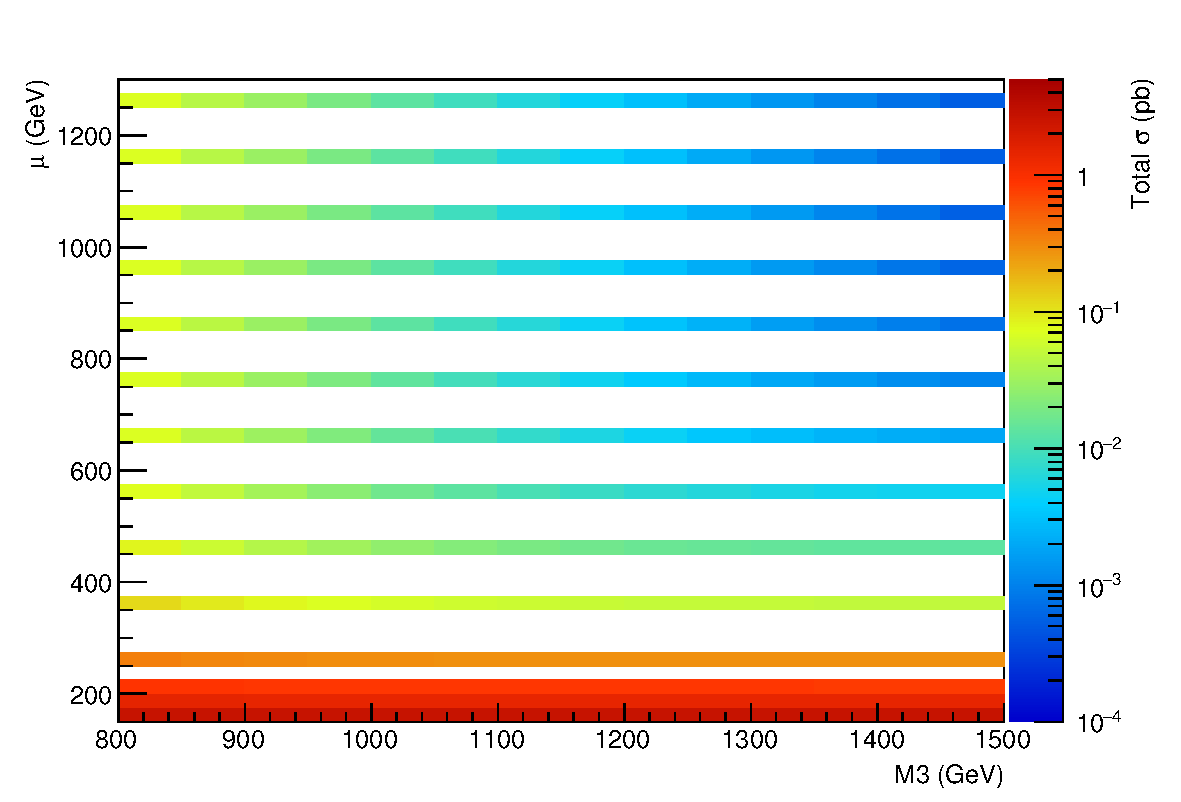
\includegraphics[width=0.49\textwidth]{figures/SigXsec_total}
  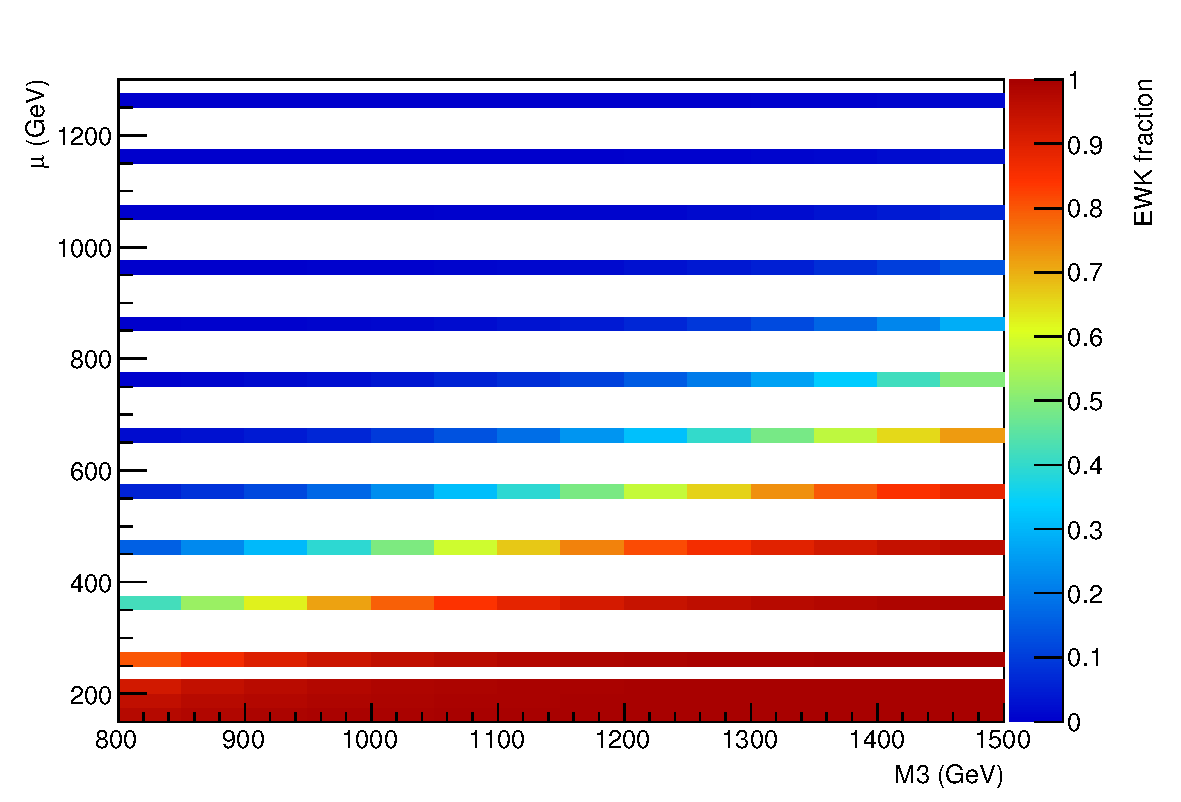
\includegraphics[width=0.49\textwidth]{figures/SigXsec_ewkFrac}
  \caption{Sección eficaz total (izquierda) y fracción relativa
    de producción electrodébil (derecha).}
  \label{fig:signal_xs_total}
\end{figure}



\subsection{Estudios a nivel generador}



\begin{figure}[!htbp]
  \centering

  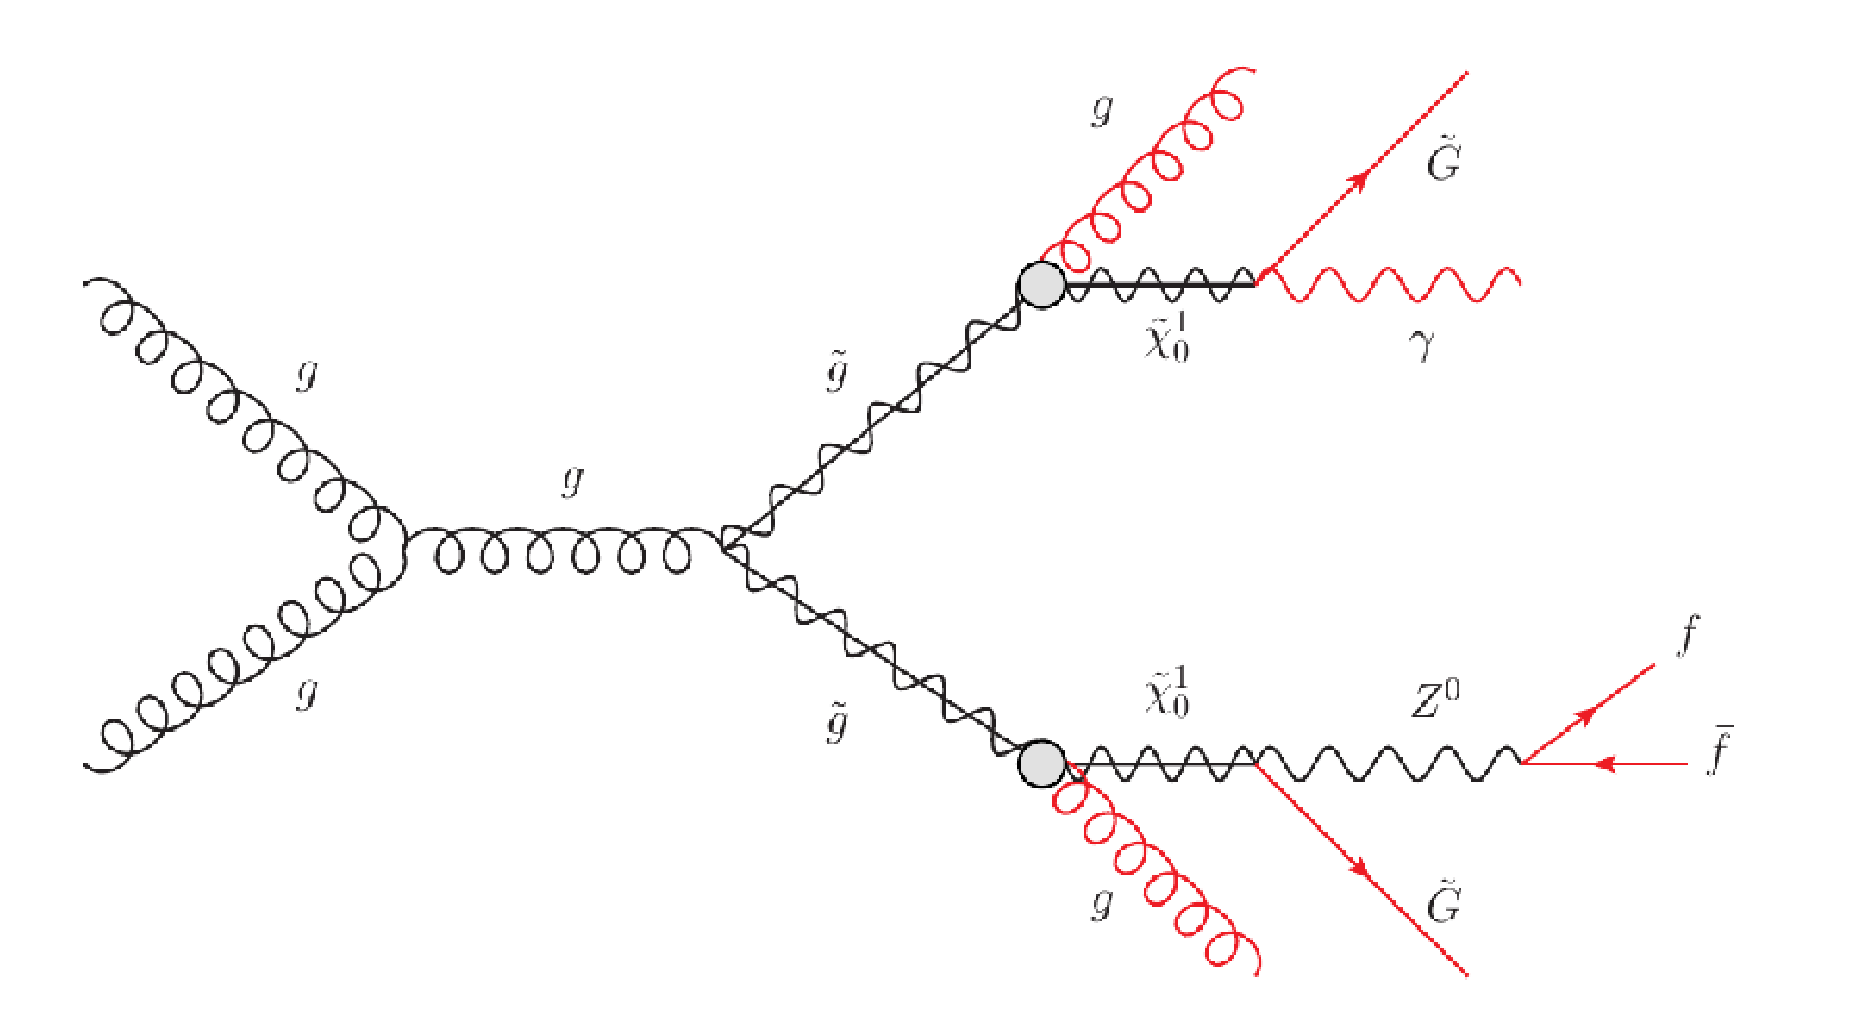
\includegraphics[width=0.49\textwidth]{diagram_a}
  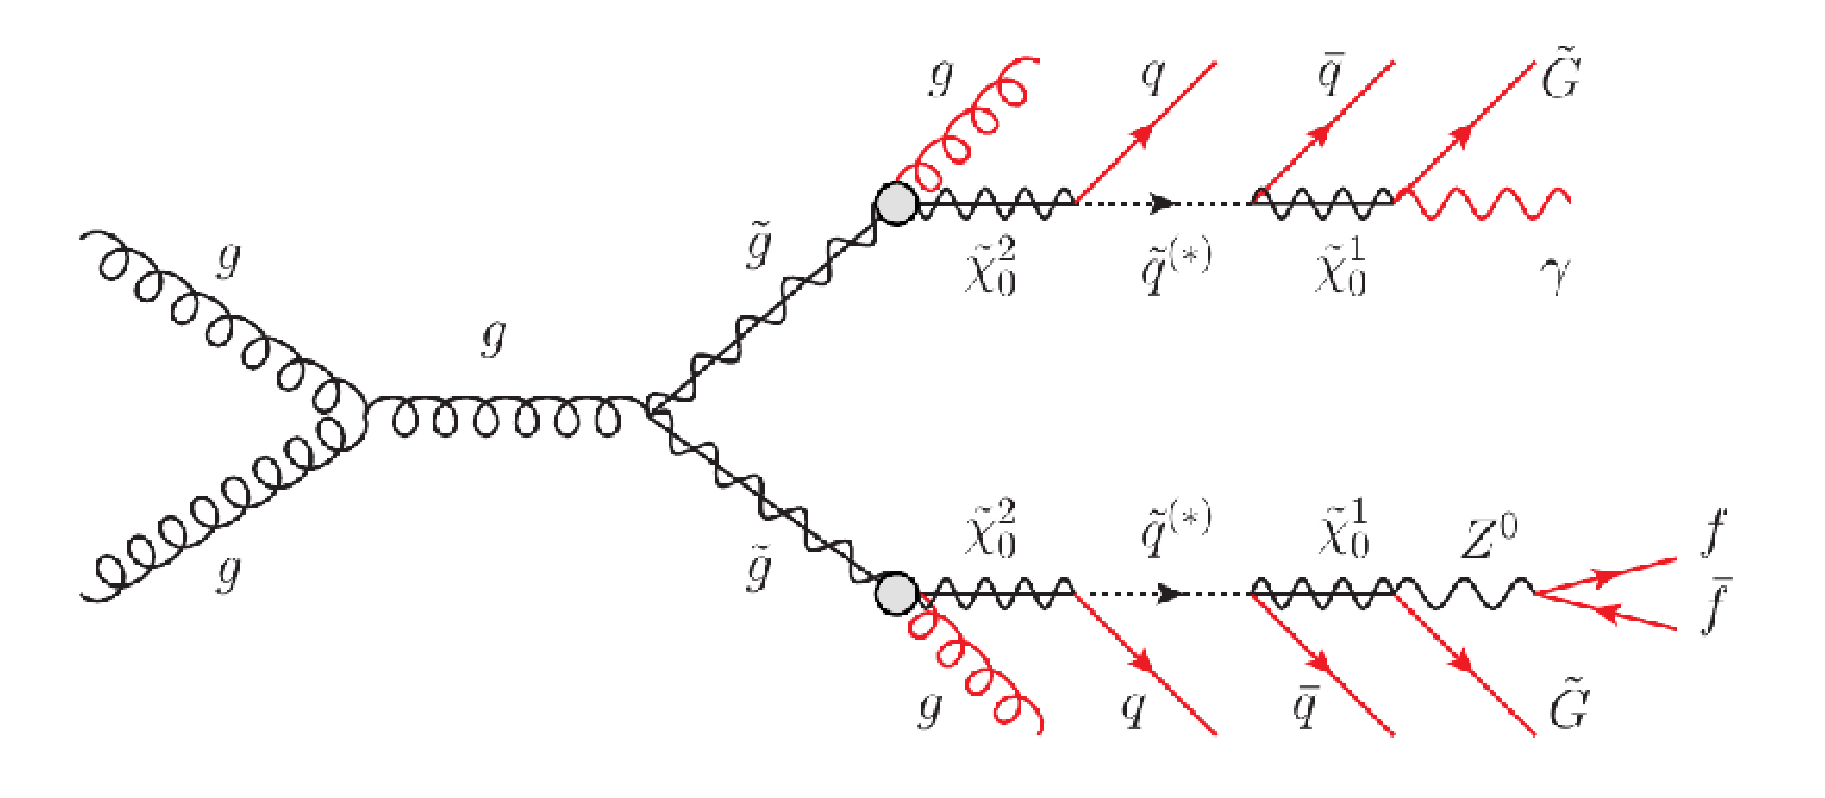
\includegraphics[width=0.49\textwidth]{diagram_b}

  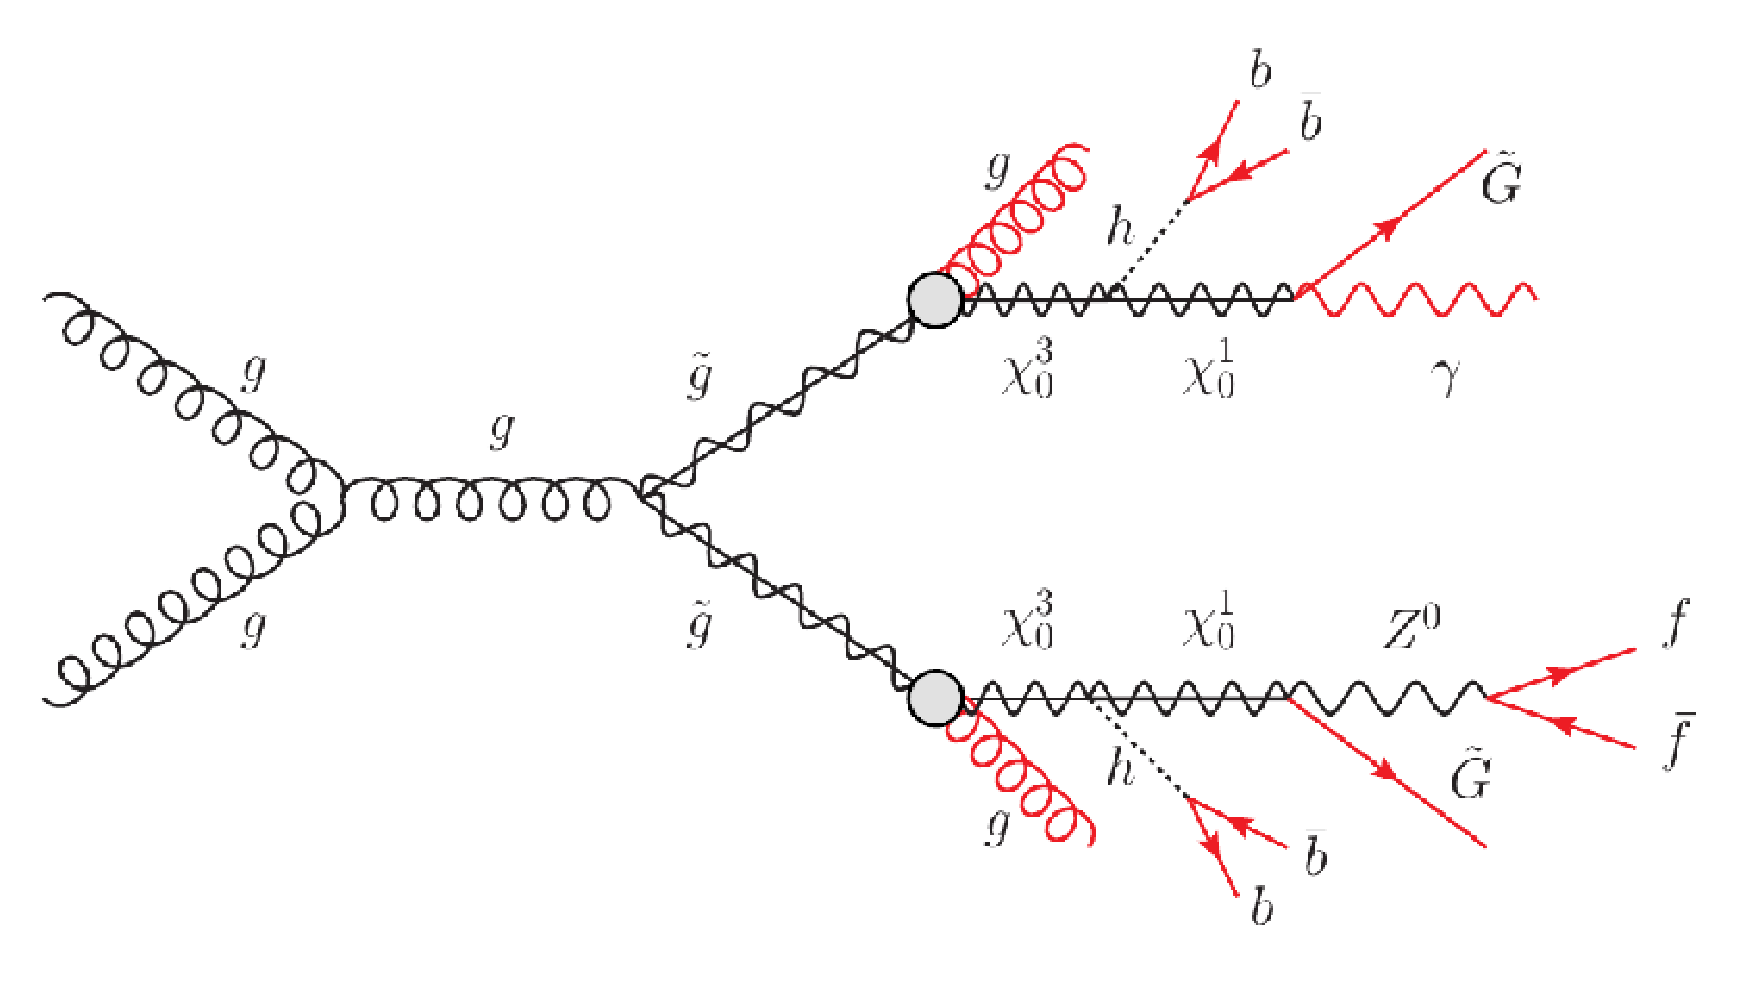
\includegraphics[width=0.49\textwidth]{diagram_c}
  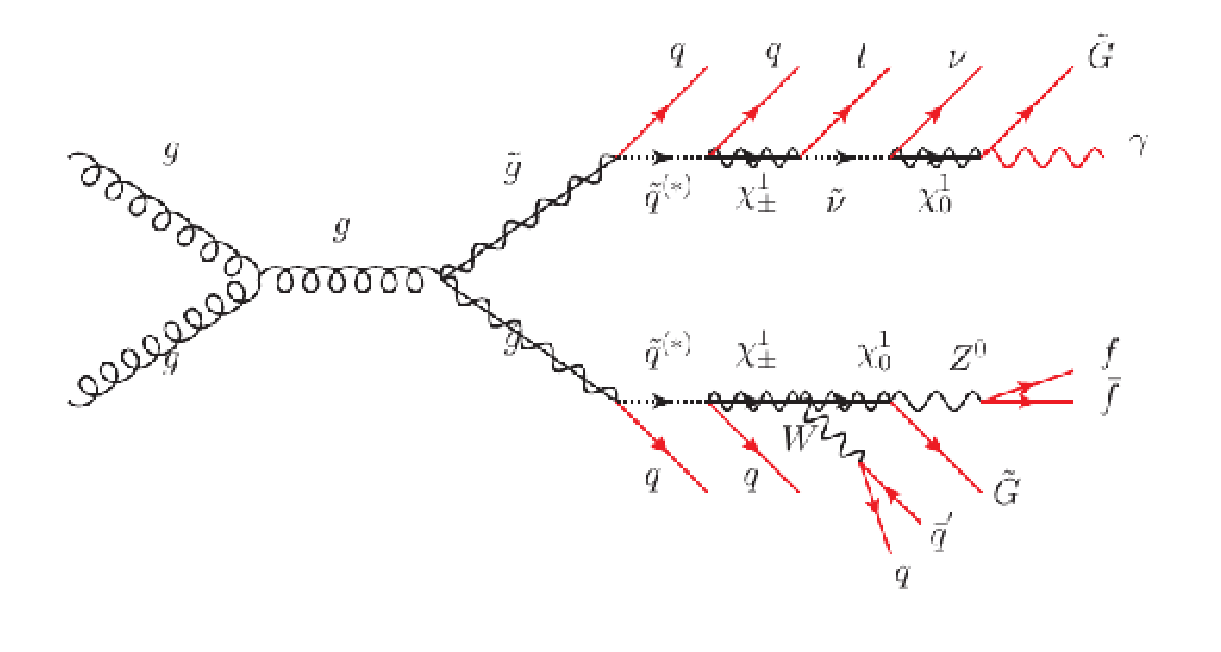
\includegraphics[width=0.49\textwidth]{diagram_d}

  \caption{...}
  \label{fig:signal_diagrams}

\end{figure}





En la \cref{fig:signal_br_n1} se observa las BR de decaimiento del
neutralino mas liviano (\ninoone). Como fue disenado las BR tienen aproximadamente
los valores descripts en \cref{eq:n1_gam,eq:n1_z,eq:nq_h}.
Estos valores varían en no más del 1\% en los distintos puntos de la grid, salvo para neutralinos
livianos ($<200\gev$) donde la producción de Higgs es altamente suprimida y
$\mathrm{BR}(\ninoone \to \gam \gravino)$ empieza a caer llegando al 40\%.
%% (ver
%% figura \cref{fig:n1_brs}).

\begin{figure}[!htbp]
  \centering

  \includegraphics[width=0.6\textwidth]{figures/br_n1_X}

  \caption{BR}
  \label{fig:signal_br_n1}
\end{figure}




\begin{figure}[h]
  \centering
  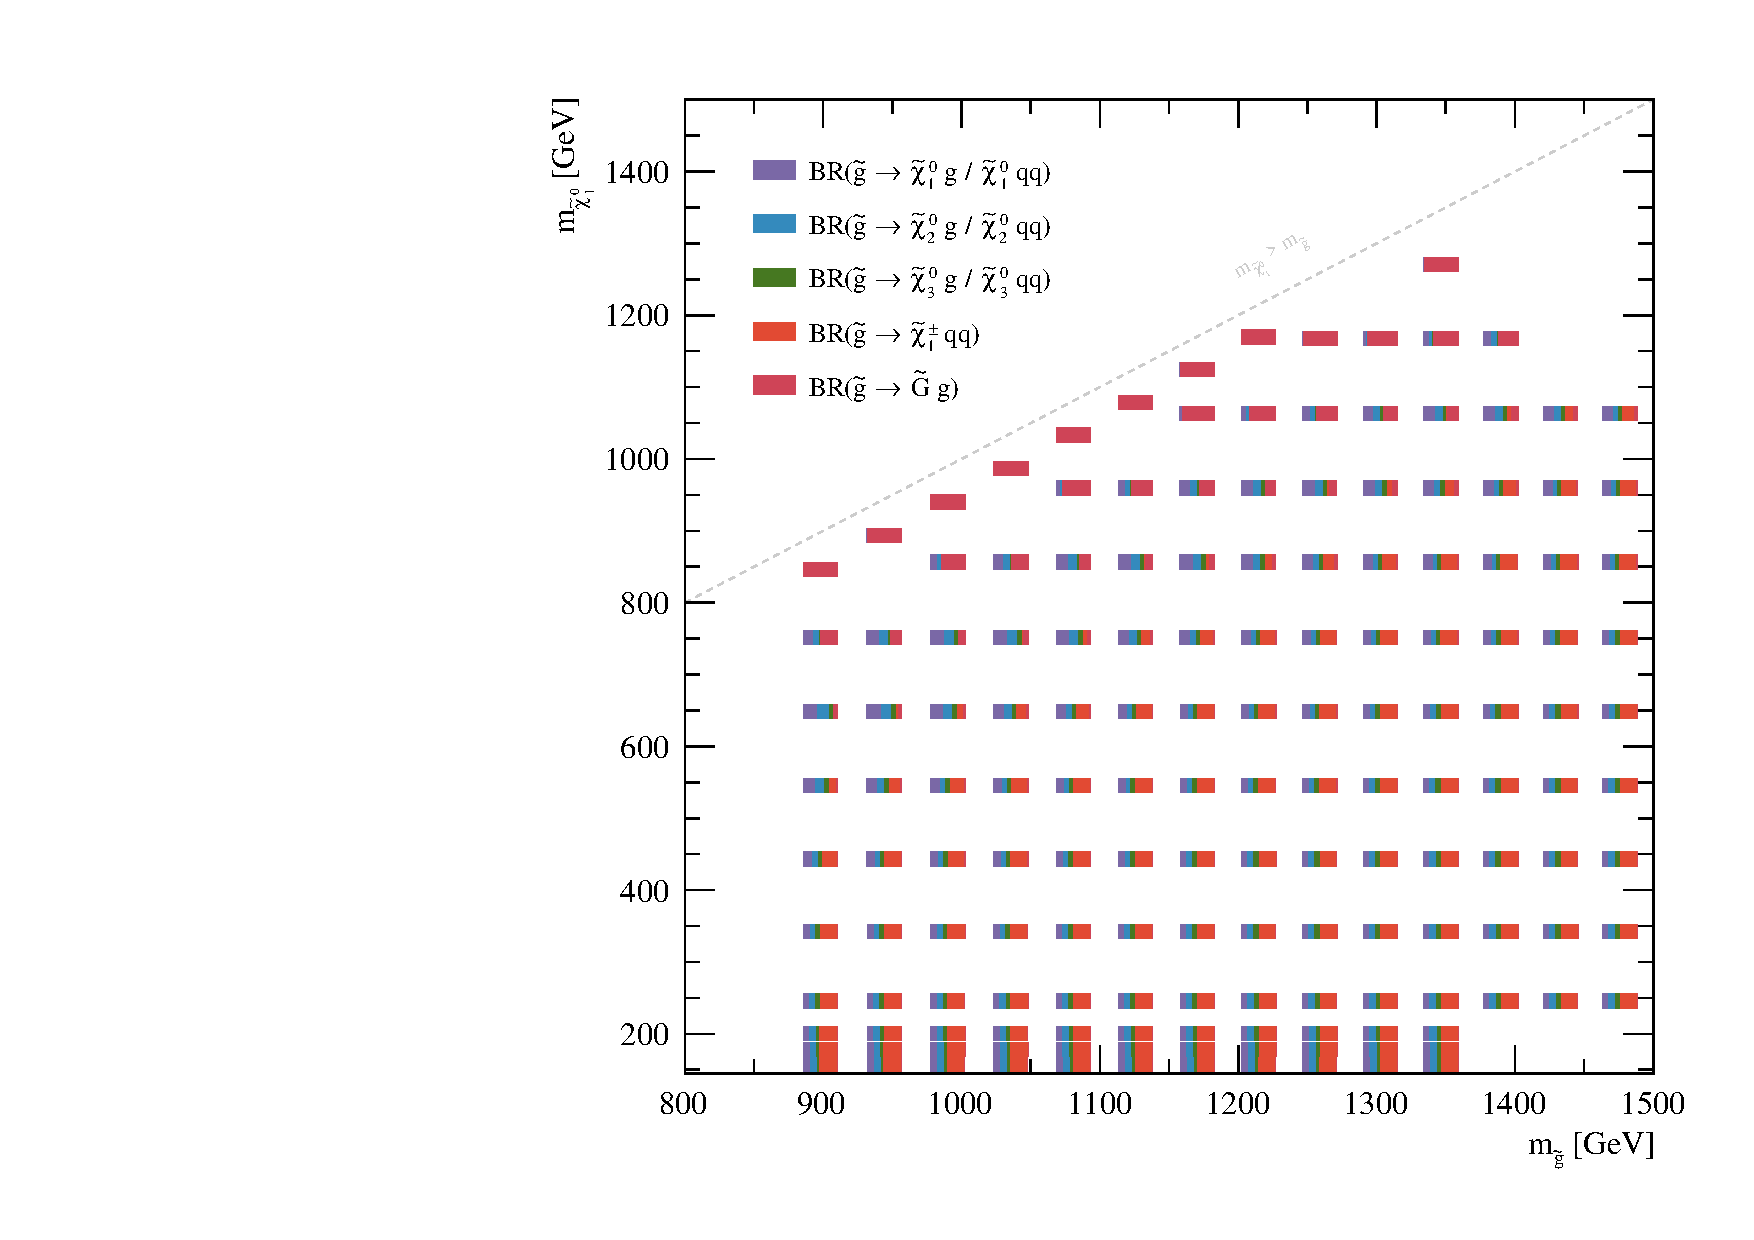
\includegraphics[width=0.8\textwidth]{figures/br_gl_X}
  \caption{BR de los gluinos para los distintos puntos de la grid.}
\end{figure}

%% \begin{figure}[h]
%%   \centering
%%   \includegraphics[width=0.8\textwidth]{figures/truth/br_gl_2b_vs_3b}
%%   \caption{BR de los gluinos para los distintos puntos de la grid.}
%% \end{figure}

%% \begin{figure}[h]
%%   \includegraphics[width=0.8\textwidth]{figures/truth/br_gl_X_2body}
%%   \includegraphics[width=0.8\textwidth]{figures/truth/br_gl_X_3body}
%%  \caption{BR de los gluinos para los distintos puntos de la grid.}
%% \end{figure}


%% \begin{figure}[h]
%%   \centering
%%   \includegraphics[width=0.8\textwidth]{figures/truth/br_c1_X}
%%   \caption{BR de los gluinos para los distintos puntos de la grid.}
%% \end{figure}

%% \begin{figure}[h]
%%   \centering
%%   \includegraphics[width=0.8\textwidth]{figures/truth/br_n3_X}
%%   \caption{BR de los gluinos para los distintos puntos de la grid.}
%% \end{figure}

%% \begin{figure}[h]
%%   \centering
%%   \includegraphics[width=0.8\textwidth]{figures/truth/br_n2_X}
%%   \caption{BR de los gluinos para los distintos puntos de la grid.}
%% \end{figure}

%% \begin{figure}[h]
%%   \centering
%%   \includegraphics[width=0.8\textwidth]{figures/truth/br_n1_X}
%%   \caption{BR de los gluinos para los distintos puntos de la grid.}
%% \end{figure}





%% %\begin{table}[ht]
%% %  \centering
%% %  \small
%% %  \begin{tabular}{|c|c|c|c|c|c|}
%% %    \hline
%% %    \hline
%% %	M3 [\gev] & $\sigma$(NLO+NLL) [\gev] & Uncertainty [$\%$] & k-factor & $m_{\neut}$ [\gev] & Filter efficiency [$\%$] \tabularnewline
%% %    \hline
%% %	\multirow{9}{*}{800} & \multirow{9}{*}{5.96 E-2} & \multirow{9}{*}{26.1} & \multirow{9}{*}{2.84} &  150 &  39.54 \\
%% %    \tiny
%% %	& & & & 175 & 44.55 \\
%% %	& & & & 200 & 47.66 \\
%% %	& & & & 250 & 55.09 \\
%% %	& & & & 350 & 65.82 \\
%% %	& & & & 450 & 71.29 \\
%% %	& & & & 550 & 73.08 \\
%% %	& & & & 650 & 69.78 \\
%% %	& & & & 750 & 47.69 \\
%% %	\hline
%% %	850 & 3.81 E-2 & 27.8 & 2.95 &  150 & 39.8 \tabularnewline
%% %	& & & & 175 & 44.6 \\
%% %	& & & & 200 &  48.4 \\
%% %	& & & & 250 &  56.0 \\
%% %	& & & & 350 &  66.1 \\
%% %	& & & & 450 &  71.4 \\
%% %	& & & & 550 &  72.5 \\
%% %	& & & & 650 &  72.0 \\
%% %	& & & & 750 &  60.2 \\
%% %	\hline
%% %	900 & 2.47 E-2 & 29.5 & 3.07 & 150 & 41.9 \tabularnewline
%% %	& & & & 175 &  46.5 \\
%% %	& & & & 200 &  50.1 \\
%% %	& & & & 250 &  56.1 \\
%% %	& & & & 350 &  64.6 \\
%% %	& & & & 450 &  71.4 \\
%% %	& & & & 550 &  73.3 \\
%% %	& & & & 650 &  73.2 \\
%% %	& & & & 750 &  66.9 \\
%% %	& & & & 850 &  34.2 \\
%% %	\hline
%% %	950 & 1.62 E-2 & 31.4 & 3.19 & 150 & 42.6 \tabularnewline
%% %	& & & & 175 &   47.5 \\
%% %	& & & & 200 &   50.6 \\
%% %	& & & & 250 &   57.1 \\
%% %	& & & & 350 &   65.8 \\
%% %	& & & & 450 &   71.8 \\
%% %	& & & & 550 &   73.7 \\
%% %	& & & & 650 &   74.1 \\
%% %	& & & & 750 &   70.4 \\
%% %	& & & & 850 &   50.7 \\
%% %	\hline
%% %	1000 & 1.08 E-2 & 33.6 & 3.33 & 150 & 43.0 \tabularnewline
%% %	& & & & 175 &   47.8 \\
%% %	& & & & 200 &   52.0 \\
%% %	& & & & 250 &    56.7 \\
%% %	& & & & 350 &    66.4 \\
%% %	& & & & 450 &    72.1 \\
%% %	& & & & 550 &    74.6 \\
%% %	& & & & 650 &    75.6 \\
%% %	& & & & 750 &    73.4 \\
%% %	& & & & 850 &    60.1 \\
%% %	& & & & 950 &    25.4 \\
%% %	\hline
%% %	1050 & 7.19 E-3 & 35.8 & 3.49 & 150 & 44.2 \tabularnewline
%% %	& & & & 175 &   48.9 \\
%% %	& & & & 200 &   52.8 \\
%% %	& & & & 250 &   58.0 \\
%% %	& & & & 350 &   66.7 \\
%% %	& & & & 450 &   72.5  \\
%% %	& & & & 550 &    74.3 \\
%% %	& & & & 650 &    76.2 \\
%% %	& & & & 750 &    74.0 \\
%% %	& & & & 850 &    66.4 \\
%% %	& & & & 950 &    41.4 \\
%% %	\hline
%% %	1100 & 4.87 E-3 & 37.8 & 3.66 & 150 & 45.5 \tabularnewline
%% %	& & & & 175 &   50.3 \\
%% %	& & & & 200 &   53.8 \\
%% %	& & & & 250 &   58.9 \\
%% %	& & & & 350 &   66.5 \\
%% %	& & & & 450 &   72.0 \\
%% %	& & & & 550 &   75.0 \\
%% %	& & & & 650 &   75.9 \\
%% %	& & & & 750 &   75.9 \\
%% %	& & & & 850 &   70.4 \\
%% %	& & & & 950 &   54.0 \\
%% %	& & & & 1050 &  19.2 \\
%% %	\hline
%% %	1150 & 3.29 E-3 & 40.0 & 3.85 &  150 & 46.3 \tabularnewline
%% %	& & & & 175 &   51.4 \\
%% %	& & & & 200 &   55.0 \\
%% %	& & & & 250 &   59.5 \\
%% %	& & & & 350 &   67.7 \\
%% %	& & & & 450 &   72.6 \\
%% %	& & & & 550 &   74.8 \\
%% %	& & & & 650 &   75.8 \\
%% %	& & & & 750 &   76.5 \\
%% %	& & & & 850 &   73.5 \\
%% %	& & & & 950 &   62.2 \\
%% %	& & & & 1050 &  31.6 \\
%% %	\hline
%% %	1200 & 2.24 E-3 & 42.3 & 4.05 &  150 & 47.1 \tabularnewline
%% %	& & & & 175 &   51.5 \\
%% %	& & & & 200 &   55.0 \\
%% %	& & & & 250 &   60.5 \\
%% %	& & & & 350 &   67.4 \\
%% %	& & & & 450 &   72.1 \\
%% %	& & & & 550 &   74.2 \\
%% %	& & & & 650 &   77.0 \\
%% %	& & & & 750 &   77.1 \\
%% %	& & & & 850 &   73.6 \\
%% %	& & & & 950 &   66.8 \\
%% %	& & & & 1050 &  45.2 \\
%% %	& & & & 1150 &  16.1 \\
%% %	\hline
%% %	1250 & 1.55 E-3 & 44.6 & 4.31 & 150 & 48.3 \tabularnewline
%% %	& & & & 175 &   52.4 \\
%% %	& & & & 200 &   56.2 \\
%% %	& & & & 250 &   60.7 \\
%% %	& & & & 350 &   67.6 \\
%% %	& & & & 450 &   72.5 \\
%% %	& & & & 550 &   74.7 \\
%% %	& & & & 650 &   77.0 \\
%% %	& & & & 750 &   77.3 \\
%% %	& & & & 850 &   75.4 \\
%% %	& & & & 950 &   70.9 \\
%% %	& & & & 1050 & 56.8 \\
%% %	& & & & 1150 & 24.9 \\
%% %	\hline
%% %	1300 & 1.07 E-3 & 46.9 & 4.56 & 150 & 49.1 \tabularnewline
%% %	& & & & 175 &   53.3 \\
%% %	& & & & 200 &   56.0 \\
%% %	& & & & 250 &   61.2 \\
%% %	& & & & 350 &   67.8 \\
%% %	& & & & 450 &   73.4 \\
%% %	& & & & 550 &   75.6 \\
%% %	& & & & 650 &   76.2 \\
%% %	& & & & 750 &   76.3 \\
%% %	& & & & 850 &   76.6 \\
%% %	& & & & 950 &   75.2 \\
%% %	& & & & 1050 & 62.7 \\
%% %	& & & & 1150 & 36.9 \\
%% %	& & & & 1250 & 16.1 \\
%% %    \hline
%% %    \hline
%% %  \end{tabular}
%% %  \caption{ The total NLO+NLL cross sections with uncertainties and K factors for GGM  signal points. The last column shows the efficiency of the generator level filter applied, to be considered for the final signal normalization.}
%% %  \label{tab:signal_xs}
%% %\end{table}


%% \begin{figure}[ht!] %  figure placement: here, top, bottom, or page
%%    \centering
%%    \includegraphics[width=0.32\textwidth]{figures/gl_n1g_full}
%%    \includegraphics[width=0.32\textwidth]{figures/gl_n1qq_full}
%%    \includegraphics[width=0.32\textwidth]{figures/gl_n1_full} \\
%%    \includegraphics[width=0.32\textwidth]{figures/gl_n2g_full}
%%    \includegraphics[width=0.32\textwidth]{figures/gl_n2qq_full}
%%    \includegraphics[width=0.32\textwidth]{figures/gl_n2_full} \\
%%    \includegraphics[width=0.32\textwidth]{figures/gl_n3g_full}
%%    \includegraphics[width=0.32\textwidth]{figures/gl_n3qq_full}
%%    \includegraphics[width=0.32\textwidth]{figures/gl_n3_full} \\
%%    \includegraphics[width=0.32\textwidth]{figures/gl_c1qq_full} \\

%%    \caption{Tasas de decaimiento para $\gluino \to \ninoone$,
%%      para todas las posibles cadenas de decaimiento permitidas en la grid
%%      de produccion fuerte. La mayoria de los graficos son la suma
%%      de deciamientos de 2 cuerpos (izquierda) y 3 cuerpos (centro).
%%      Para el decaimiento $\gluino \to \chinopm$), solo el decaimiento de
%%      tres cuerpos es posible.}
%%    \label{fig:br_gl_n1}
%% \end{figure}

%% \clearpage

%% \begin{figure}[ht!]
%%   \centering
%%   \includegraphics[width=0.5\textwidth]{figures/GGM_xs_vs_M3}
%%   \caption{Seccion eficaz de produccion de pares de gluinos como funcion de la masa del gluino, calculada a NLO+NLL con {\nllfast}\hl{fix}.}
%%   \label{fig:signal_xs_vs_M3}
%% \end{figure}
